\section{Approach}
\label{sec:approach}
In this section, we first present two simple but effective style transfer models, namely \emph{CrossAlign}~\cite{shen2017style} and \emph{VAE}~\cite{john2018disentangled} as our base models, and then present a meta-learning framework called model-agnostic meta-learning~\cite{finn2017model} that incorporates the base models to solve the few-shot style transfer problem.

\subsection{Preliminaries}
%Compared with methods that require multiple layers of operations 
%such as the \emph{Delete-and-Retrieve}~\cite{li2018delete}, 
%much state-of-the-art work use specific model designs to disentangle the style 
%and content in latent space, and used a single-layer model structure. 
%We briefly present two successful single-layer models below.
%Therefore, they are a simple and effective starting point to explore meta-learning framework for the style transfer task. We adapt the \emph{Model Agnostic Meta-learning} scheme on the \emph{CrossAlign} model and \emph{VAE} model in our study~\cite{shen2017style, john2018disentangled}.
%
\subsubsection*{Cross Align}

The \emph{CrossAlign} model architecture proposed by \citet{shen2017style} is shown in \figref{fig:crossalign}. Let $X$ and $Y$ be two corpora with styles $s_x$ and $s_y$, respectively. $E$ and $D$ are encoders and decoders that take both the sentence $x$ or $y$, and their corresponding style labels $s_x$ or $s_y$ as inputs. Then the encoded sentences $z_x$ and $z_y$, together with their labels are input to two different adversarial discriminators $D_1$ and $D_2$, which are trained to differentiate between logits generated by the concatenation of content embedding and the original/opposite style label.

\begin{figure}[htbp]
	\centering
	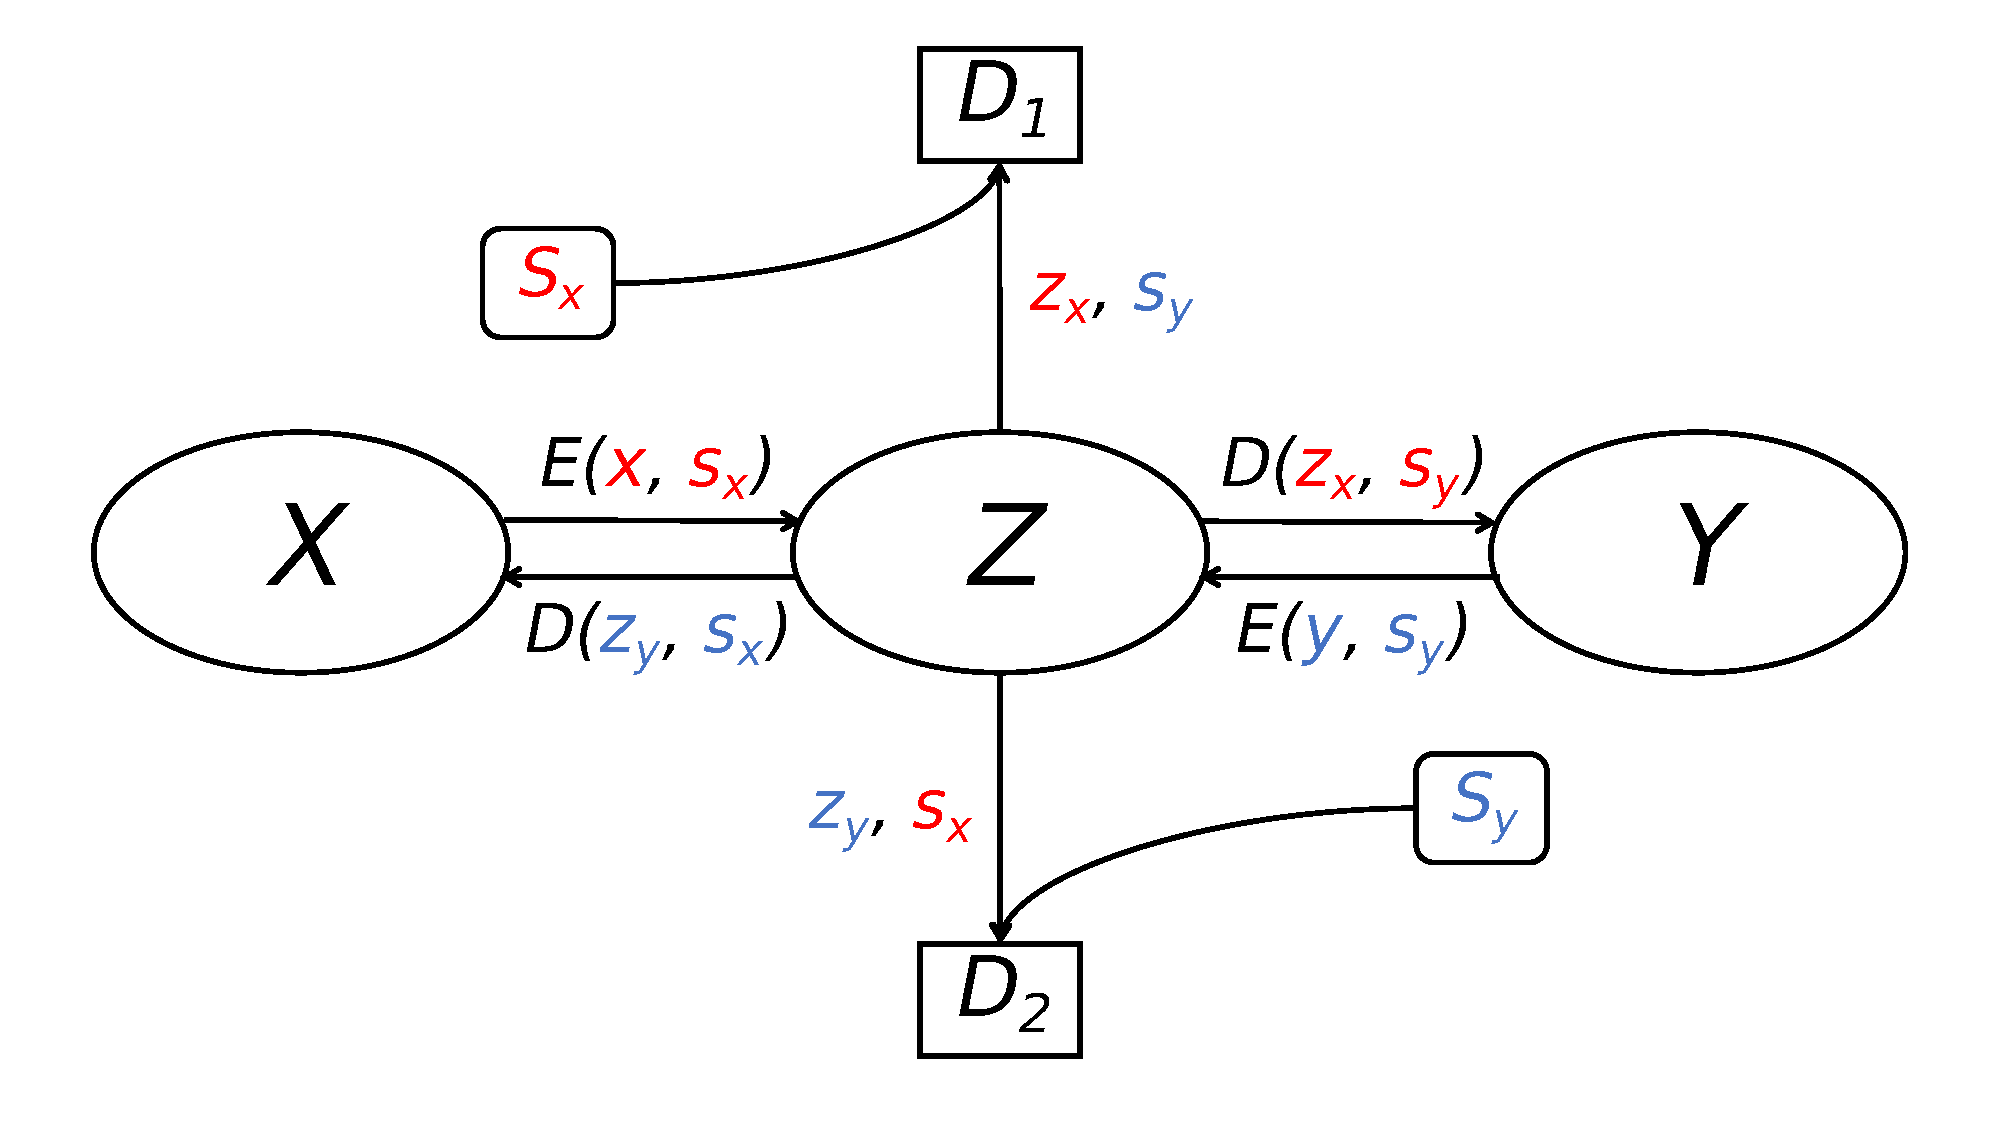
\includegraphics[width=7cm]{./images/crossalign.pdf}
	\caption{CrossAlign architecture}
	\label{fig:crossalign}
\end{figure}

\XQ{I think explaining what the loss function is designed for in words is better than showing the formula.}
In training phase, the discriminators and the seq2seq model are trained jointly. The objective is to find
\begin{align*}
\theta^* = \underset{\theta}{\arg\min\ } \mathcal{L}_{\mathrm{rec}} (\theta_E, \theta_D) + \mathcal{L} _{\mathrm{adv}}(\theta_E, \theta_D),
\end{align*}
where
\begin{align*}
\mathcal{L}_{\mathrm{adv}}(\theta_E, \theta_D) & = \mathbb{E}_{x\sim X}[-\log D(E(x, s_x))] & \\
& + \mathbb{E}_{y\sim Y}[-\log (1 - D(E(y, s_y)))].
\end{align*}
The discriminators are implemented as CNN classifiers~\cite{kim2014convolutional}.


\subsubsection*{VAE for Style Transfer}

In order to disentangle style and content in the latent space, \citet{john2018disentangled} used variational autoencoder (VAE) and their specially designed style-oriented and content-oriented losses to guide the updates of the latent space distributions for the two components~\cite{kingma2013auto}. 

The architecture of this model is shown in \figref{fig:vae}. Given a corpus $X$ with unknown latent style space and content space, 
an RNN encoder maps a sequence $x$ into the latent space, 
which defines a distribution of style and content~\cite{cho2014learning}. 
Then style embedding and content embedding are sampled from 
their corresponding latent distributions and are concatenated 
as the training sentence embedding. 

The two embeddings are used to calculate multi-task 
loss $J_{\mathrm{mul}}$ and adversarial loss $J_{\mathrm{adv}}$ 
for content and style to separate their information. 
Then this concatenated latent vector is used as a generative 
latent vector, and is concatenated to every step of the input sequence
and fed into decoder $D$, which reconstructs the sentence $x'$. 
The final loss is the sum of these multi-task losses and the usual VAE reconstruction $J_{\mathrm{rec}}$ with 
KL divergence for both style embedding and content 
embedding~\cite{kingma2013auto}.

\begin{figure}[htbp]
	\centering
	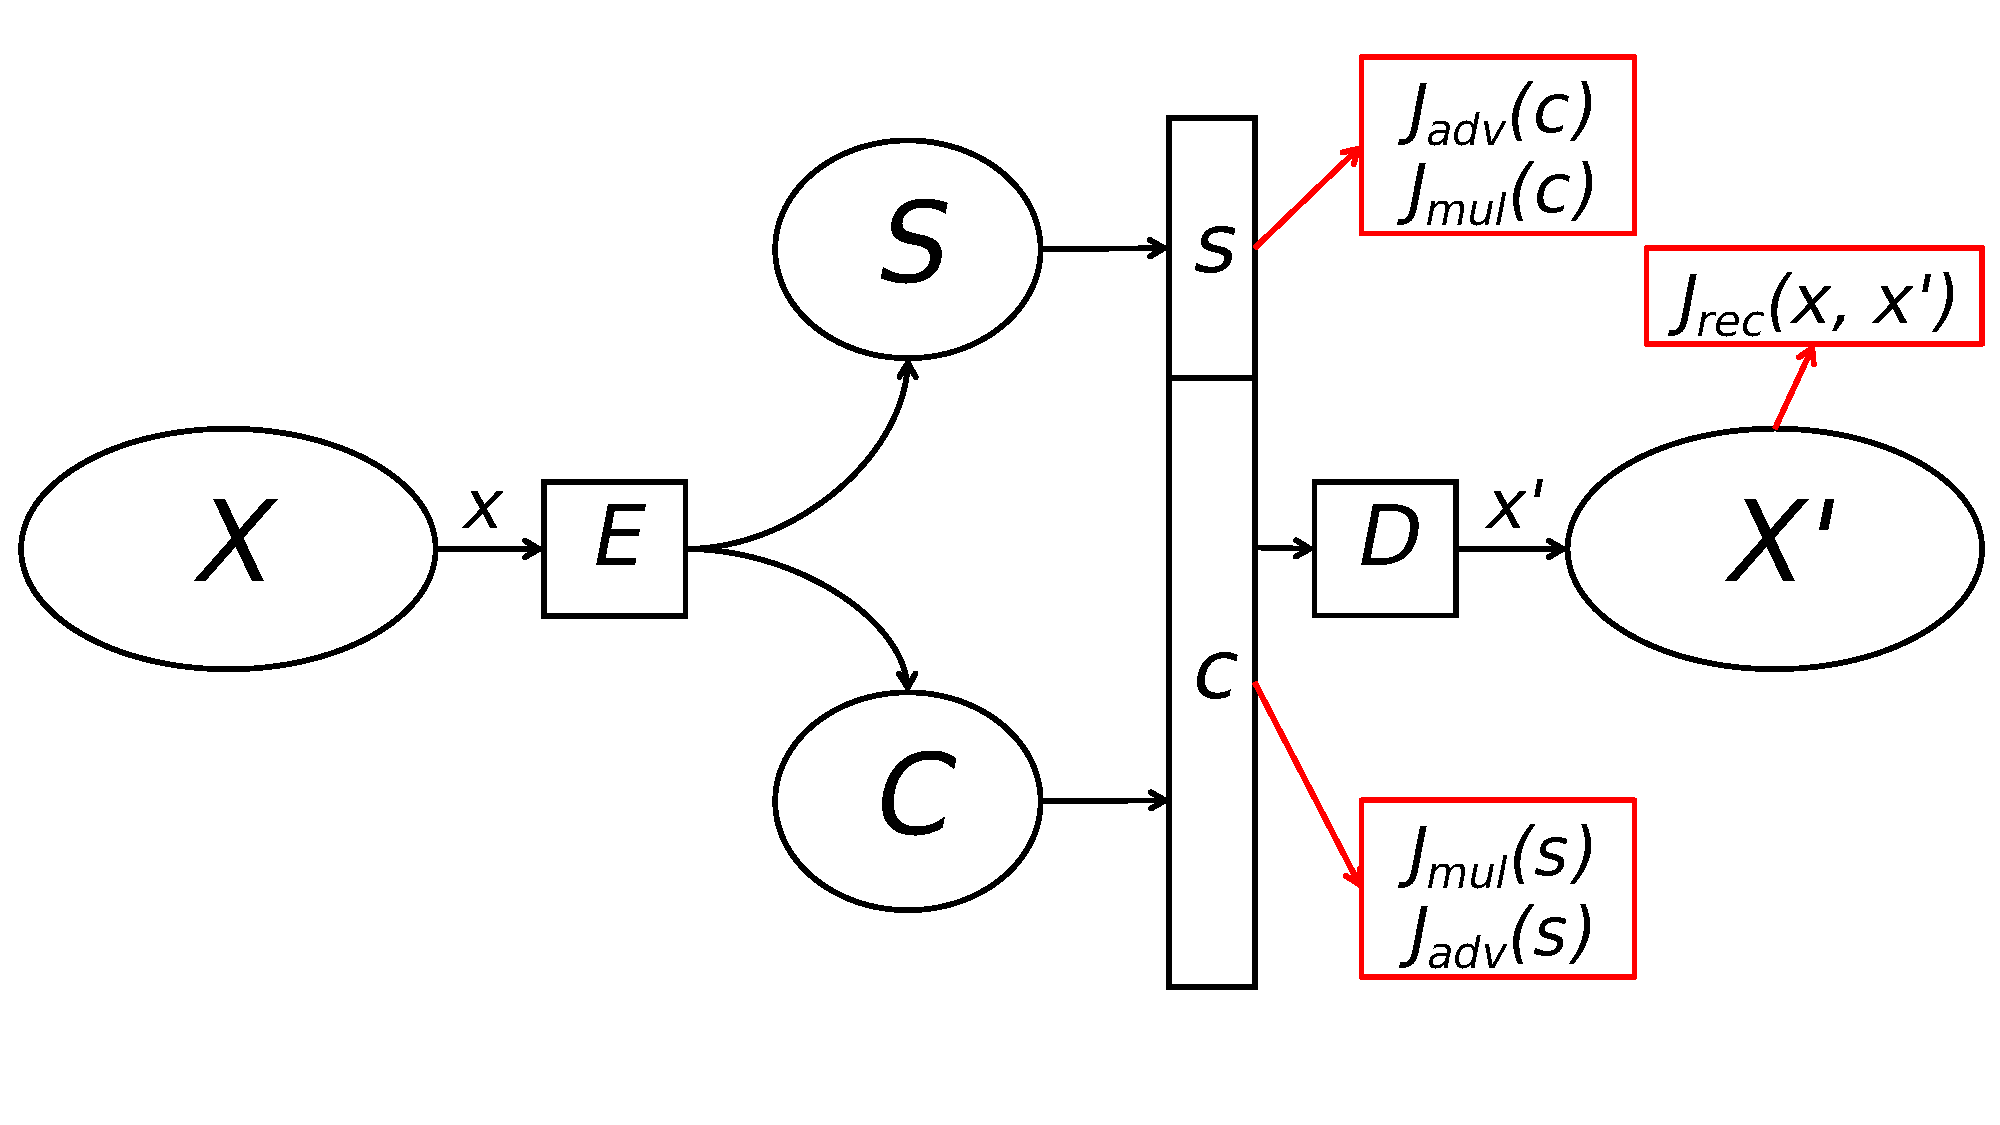
\includegraphics[width=7cm]{./images/vae.pdf}
	\caption{VAE architecture}
	\label{fig:vae}
\end{figure}


%The main designs of style- and content-oriented losses are as 
%follows~\cite{john2018disentangled}.
%\begin{enumerate}
%	\item The style embedding should contain enough information to be discriminative. Therefore, a multitask discriminator is added to align the predicted distribution and the ground-truth distribution of labels.
%	\begin{align*}
%	J_{\mathrm{mul}}(\theta_E; \theta_{\mathrm{mul(s)}}) = -\sum_{l\in \mathrm{labels}}t_s(l)\log y_s(l),
%	\end{align*}
%	where $t_s(l)$ is the distribution of ground-truth style labels, and $y_s(l)$ is the predicted output by the style discriminator.
%	\item The content embedding should not contain too much style information. Therefore, an adversarial discriminator is added, with loss of the discriminator and adversarial loss for the autoencoder given by
%	\begin{align*}
%	J_{\mathrm{dis}(s)}(\theta_{\mathrm{dis}(s)}) & = - \sum_{l\in \mathrm{labels}} t_s(l)\log y_s(l), \\
%	J_{\mathrm{adv(s)}}(\theta_E) & = -\sum_{l\in \mathrm{labels}}y_s(l)\log y_s(l),
%	\end{align*}
%	where $\theta_{\mathrm{dis}(s)}$ contains the weights for a fully connected layer, and $t_c(l)$ is the predicted distribution of style labels when taking content embedding as an input. 
%	\item The content embedding needs to be able to predict the information given by bag-of-words (BoW), which is defined as
%	\begin{align*}
%	t_c(w) := \frac{\sum_{i=1}^N \mathbb{I}\{w_i = w \}}{N},
%	\end{align*}
%	for each word $w$ in the vocabulary $V$ with sentence length $N$~\cite{wallach2006topic}. Therefore, a multitask discriminator is added to align the predicted BoW distribution with ground-truth.
%	\begin{align*}
%	J_{\mathrm{mul}(c)}(\theta_E; \theta_{\mathrm{mul}(c)}) & = -\sum_{w\in V}t_c(w)\log y_c(w),
%	\end{align*}
%	where $t_c(w)$ is the distribution of true BoW representations, and $y_c(w)$ is the predicted output by the content discriminator.
%	\item The style embedding should not contain content information. Similar as before, an adversarial discriminator is trained to predict the BoW features from style embedding, with loss for discriminator and adversarial loss given by
%	\begin{align*}
%	J_{\mathrm{dis}(c)}(\theta_{\mathrm{dis}(c)}) = -\sum_{w\in V}t_c(w)\log y_c(w), \\
%	J_{\mathrm{adv}(c)}(\theta_E) = -\sum_{w\in V}y_c(l)\log y_c(l).
%	\end{align*}
%\end{enumerate}


In the training phase, the adversarial discriminators are trained 
together with other parts of the model, and the final loss of 
the autoencoder is given by the weighted sum of the loss from traditional VAE, 
the multitask losses for style and content, 
and the adversarial losses given by the style and content discriminators. 
Then in the inference phase, the style embedding is extracted from the 
latent space of a target domain, and the original style embedding is 
substituted by this target embedding in decoding.

\subsection*{Model-Agnostic Meta-learning (MAML)}

Meta-learning is designed to help a model quickly adapt to a new tasks, given that it has been trained on several other similar tasks. Compared with other model-based meta-learning methods, model-agnostic meta-learning algorithm (MAML) utilizes only gradient information~\cite{finn2017model}. Therefore, it can be easily applied to models based on gradient descent training.

Given a distribution of similar tasks $p(\mathcal{T})$, a task-specific loss function $\mathcal{L}_{\mathcal{T}_i}$ and shared parameters $\theta$, we aim to jointly learn a model so that in fine-tuning with the new task, the parameters are well-initialized so that the model quickly converges with fewer epochs and a smaller dataset.

Figure \ref{fig:maml} shows the architecture of MAML. We define the shared model with parameters $\theta$ as a meta-learner. The data for each task is divided in to a support set $D_s$ and a query set $D_q$. Every update of the meta-learner's parameters consist of $K$-step updates for each of the $N$ tasks. The support set for each task is used to update the $N$ sub-tasks, and the query set is used to evaluate a query loss that is later used for meta-learner's updates.

In each sub-task training, the sub-learner is initialized with the parameters of the meta-learner. Then this parameter is updated $K$ times using the support data for this specific task. After updating, the new parameter is $\theta'_i$ for the $i$-th task, and a loss $\mathcal{L}_{\mathcal{T}_i}(f_{\theta'})$ is evaluated using the query dataset for this sub-task. This sub-training process is performed for each sub-task, and losses from all sub-tasks are aggregated to obtain a loss for meta-training.

\begin{figure}[th]
	\centering
	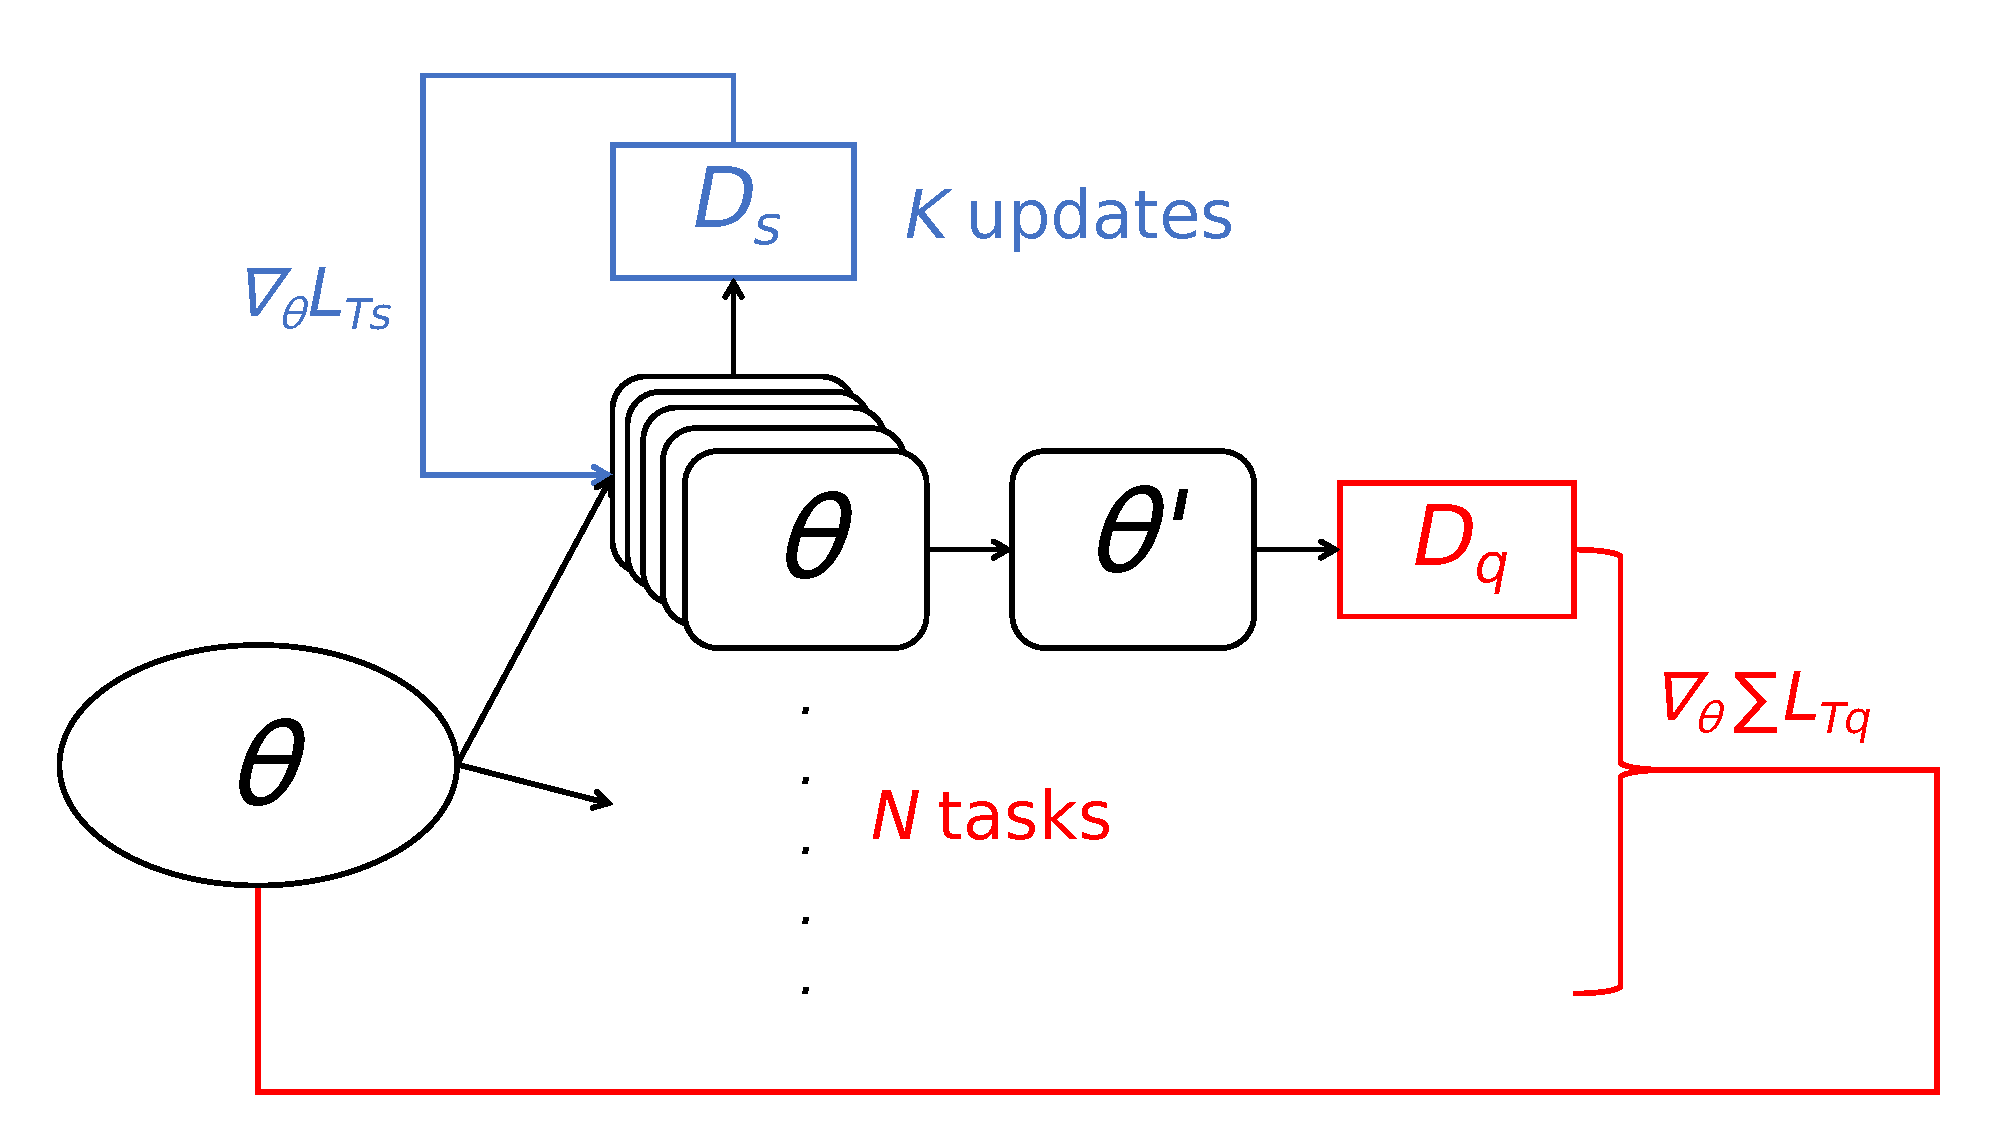
\includegraphics[width=7cm]{./images/maml.pdf}
	\caption{MAML architecture. For every update of meta-learner's parameters $\theta$, we first update each sub-task on the support dataset $D_s$ for $K$ steps and obtain the new parameter $\theta'$. Then we use the loss evaluated using this new parameter on the query set $D_q$, and sum up all losses from $N$ tasks to update meta-learner's parameters.}
	\label{fig:maml}
\end{figure}

\begin{algorithm}\small
	\caption{ST$^2$}
	\label{alg:maml}
	\KwIn{a set of style pairs, $\{(s_{t,1}, s_{t,2}), \ldots \}$, where $t = 1, \ldots, N$, parameters $\alpha, \beta$}
	\KwOut{transfer function $f_{\theta}: (x, s) \mapsto y$, where $s$ is the source style, $x$ is the original sentence, $y$ is the transferred sentence in target style}
	\While{not done}{
		\ForEach{style pair $(s_{t,1}, s_{t,2})$}{
			Initialize sub learner with $\theta_t = \theta$\;
			\For{step in 1, \ldots, K}{
				Sample batch data from support set of $t$\;
				Update transfer function $f_{\theta}$ using\\$\qquad\theta_t = \theta_t - \alpha \nabla_{\theta_t}\mathcal{L}_{t}(f_{\theta_t})$\;
			}
			Sample batch data from query set of $t$\;
			Evaluate $\mathcal{L}_t(f_{\theta_t})$\;
		}
		Update meta-learner with $\theta = \theta - \beta\nabla_{\theta}\sum_{t=1}^T \mathcal{L}_t(f_{\theta_t})$\;
	}
\end{algorithm}

\subsection{ST$^2$}

In our application, the sub-tasks contain different pairs of styles to 
be transferred. The meta-learner contains the transfer function 
$f_{\theta}: (x, s)\mapsto x'$, which takes a sentence $x$ with its 
style label $s$, and outputs a sentence $x'$ in the target style with 
similar content. This transfer function is shared by all pairs of styles 
in the meta-training phase. In addition, both our base models include adversarial functions for style disentanglement, the updates for the adversarial parameters are also included in the updates of meta-learner. Since the data size for each task with a 
single pair of styles is assumed to be small, 
the goal of MAML is to use information from other style pairs for 
a better initialization in the fine-tuning phase of a specific sub-task. 
The multi-task style transfer via meta-learning (ST$^2$) algorithm is 
described in Algorithm \ref{alg:maml}. 
